\documentclass[a4paper]{article}
\usepackage{graphicx}
\usepackage{twocolceurws}


\title{Homework 1: Computing Pi in Serial and Parallel}

\author{
Stella Greenvoss \\ 
10/29/2025 | CS431\\
All computation done on ix-dev
}

\begin{document}
\maketitle

In this report, three different methods of computing pi with varying degrees of parallelism will be briefly analyzed both in terms of their runtime at different numbers of steps (N) and their distance from actual pi at each given N. Note that all graphs have logarithmic scales on both their X- and Y-axes.
\section{Runtime}
First, the runtime of the different methods will be discussed.
\subsection{Serial}
Per the instructions, the first step of this project is to compute pi serially. We were instructed to use the method of integration, as written below.
\begin{verbatim}
double calcPi_Serial(int num_steps)
{
    double pi = 0.0;
    double line_seg = 1.0 / num_steps;
    for (int i = 0; i < num_steps; i++) {
        double left_end = (double) i / 
            num_steps;
        double y = sqrt(1.0 - 
            (left_end * left_end));
        pi += (y * line_seg) * 2;	
    }
    return pi * 2;
}
\end{verbatim}
This function takes as an argument the number of steps that the integration approximation should take, and returns the approximate value of pi.

This program runs relatively quickly at very high scales. As seen in Figure 1, the execution time at $10^8$ loop iterations is still under one second. This was unexpected for me, as I expected the serial algorithm to be profoundly worse at these large scales; it is worse when compared to the parallelized results, but the execution time is still quite good. This can likely be attributed to the -O3 optimization flag set in the Makefile. 

\begin{figure}[ht]
\begin{center}
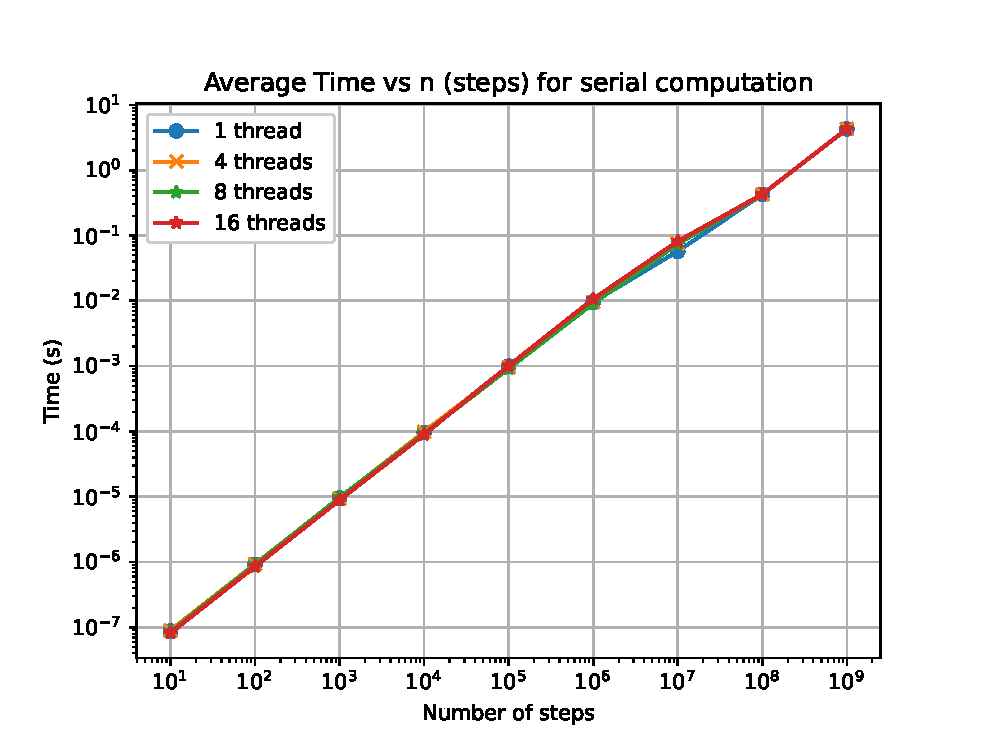
\includegraphics[height=6cm]{fig_serial.eps}
\caption{Serial results at the four thread counts averaged over five runs at each count. The lines are on top of one another: thread count has no impact.}
\label{fig1}
\end{center}
\end{figure}

It is unsurprising to note that the number of threads had no significant impact on the execution time, since this function is designed to run serially.  

\subsection{Parallel 1: Integration}
The next function uses the same method as the serial integration-based estimation of pi but uses an OpenMP compiler directive to enable parallelism. 

\begin{verbatim}
double calcPi_P1(int num_steps)
{
    double pi = 0.0;
    double line_seg = 1.0 / num_steps;
    
    #pragma omp parallel for reduction(+:pi)
    for (int i = 0; i < num_steps; i++) {
            ... 
            program continues as before 
\end{verbatim}

When attempting to parallelize, I tried to use a simple parallel for directive while treating the pi as an atomic variable, but found that this consistently worked to bottleneck execution time to the point where this function was running much slower than the serial version. 

Instead, a better approach is to use OpenMP's built-in solution for accruing a value over a number of loops: the reduction clause. Applying this allowed for the speedup that is made clear by Figure 2. 

\begin{figure}[ht]
\begin{center}
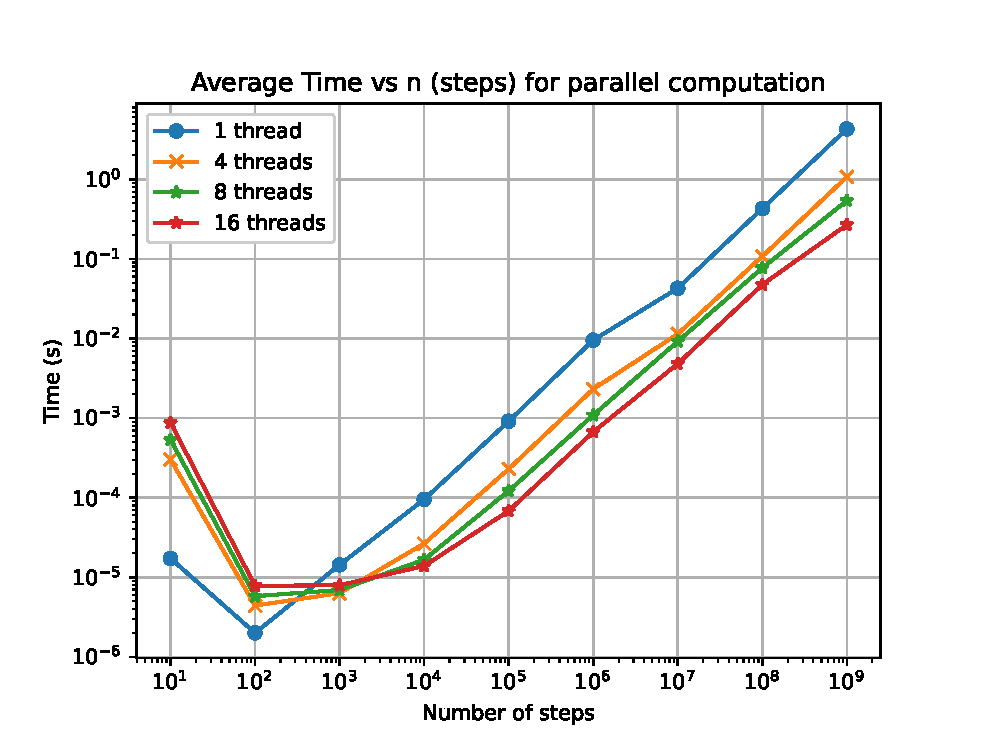
\includegraphics[height=6cm]{paral1.eps}
\caption{Parallel results at the four thread counts, averaged over five runs at each count.}
\label{fig2}
\end{center}
\end{figure}

The initial spike at a small value of n probably reflects the overhead from parallelism, and might explain why the blue line (describing the average execution time when there is one thread) is initially much lower than the others. Quickly, however, the multi-threaded processes run much faster than the single-threaded one, with 16 threads being the most performant configuration. 


\subsection{Parallel 2: Monte Carlo}
Finally, the Monte Carlo method was used to approximate pi. This method consists of generating two random numbers in [0..1], then checking whether they fall within a unit circle's first quadrant. This can be parallelized using more OpenMP compiler directives. 
\begin{verbatim}
double calcPi_P2(int num_steps)
{
	double x, y;
	int sum;
	unsigned int seed;

	#pragma omp parallel private(x, y, seed)
	{
		seed = omp_get_thread_num();
	
		#pragma omp for reduction(+:sum)
		for (int i = 0; i < num_steps; i++) {
			x = (double) rand_r(&seed) / RAND_MAX;
			y = (double) rand_r(&seed) / RAND_MAX;
			if ((x*x + y*y) <= 1) sum += 1;
		}
	} 
	return 4 * 
        ((double)sum / (double)num_steps);	
}
\end{verbatim}

Making the enclosing scope of the parallelized for loop also parallel, with each variable (excluding sum) being private, ended up being key to optimizing this function. It was also clear that the reduction in this case also works better than making the sum an atomic variable, and that the thread-safe rand\_r is far better than using the regular rand function. 

\begin{figure}[ht]
\begin{center}
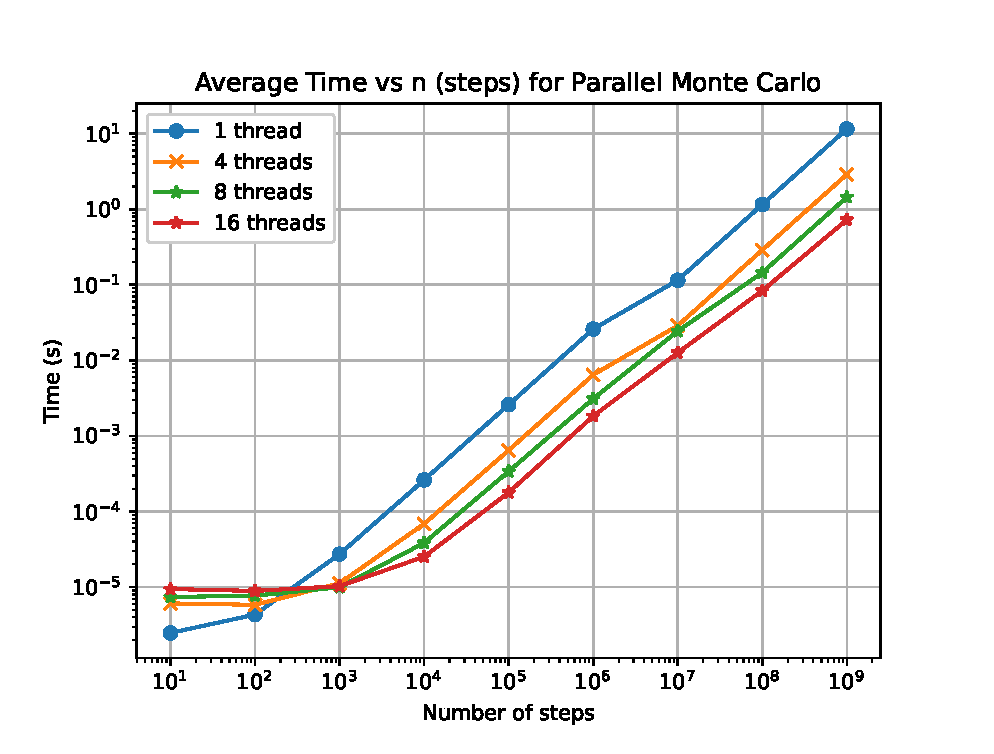
\includegraphics[height=6cm]{carlo.eps}
\caption{Parallelized Monte Carlo results at the four thread counts, averaged over five runs at each count.}
\label{fig3}
\end{center}
\end{figure}

This graph looks similar to the graph for the parallelized integration function, with slight differences. For one, the efficiency spike for single-threaded processes running on small n is still present, but is less dramatic, since higher thread counts do not take as much of a performance hit as in the other parallel function. 

\section{Accuracy}
The following graph shows the accuracy for each of the three different methods at different thread counts and at different n.
\begin{figure}[ht]
\begin{center}
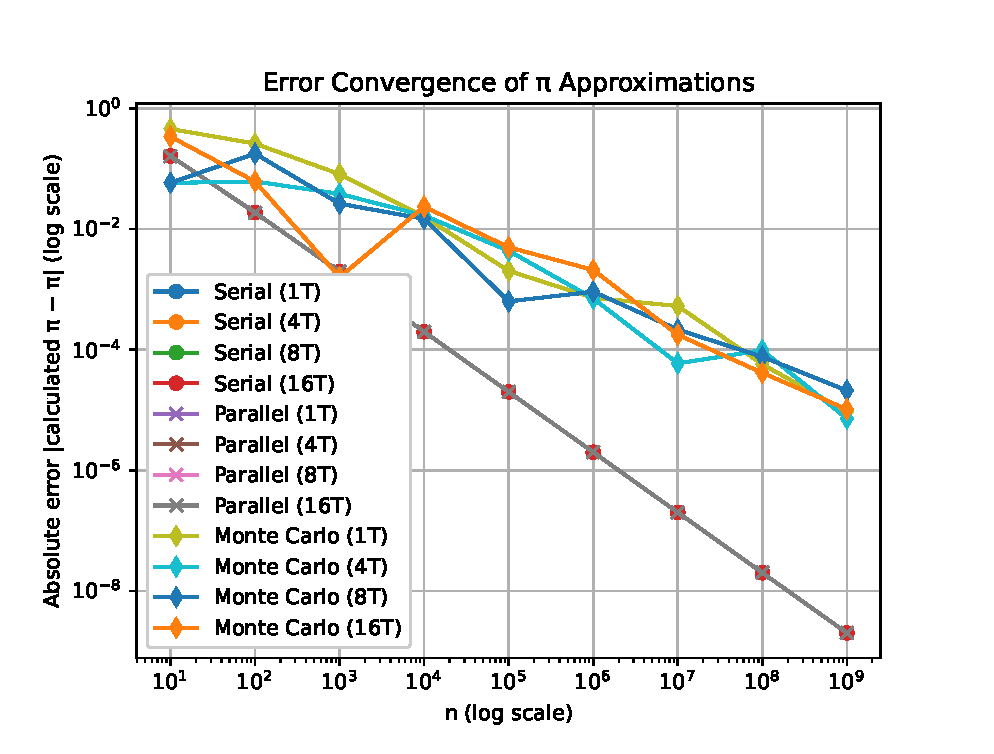
\includegraphics[height=6cm]{errs.eps}
\caption{The absolute error of the estimated pi value for each of the three different functions.}
\label{fig4}
\end{center}
\end{figure}
Thread count has no impact on either of the integration-based functions' accuracy. Upon reflection, this is obvious; since they both perform the same mathematical operation, they will both compute the same value of pi for each n. However, the Monte Carlo method 's accuracy seems to vary between thread counts. Whether this is because of the inherent randomness within the Monte Carlo method - or if it can be described as a true converging pattern toward consistent predictions at different thread counts - requires more investigation and is beyond the scope of this initial exploration. Suffice it to say that the Monte Carlo method is by far the least efficient at computing pi with accuracy for these values of n. 

\section{Speedup}
The speedup of the two parallel methods is shown in figure 5.
\begin{figure}[ht]
\begin{center}
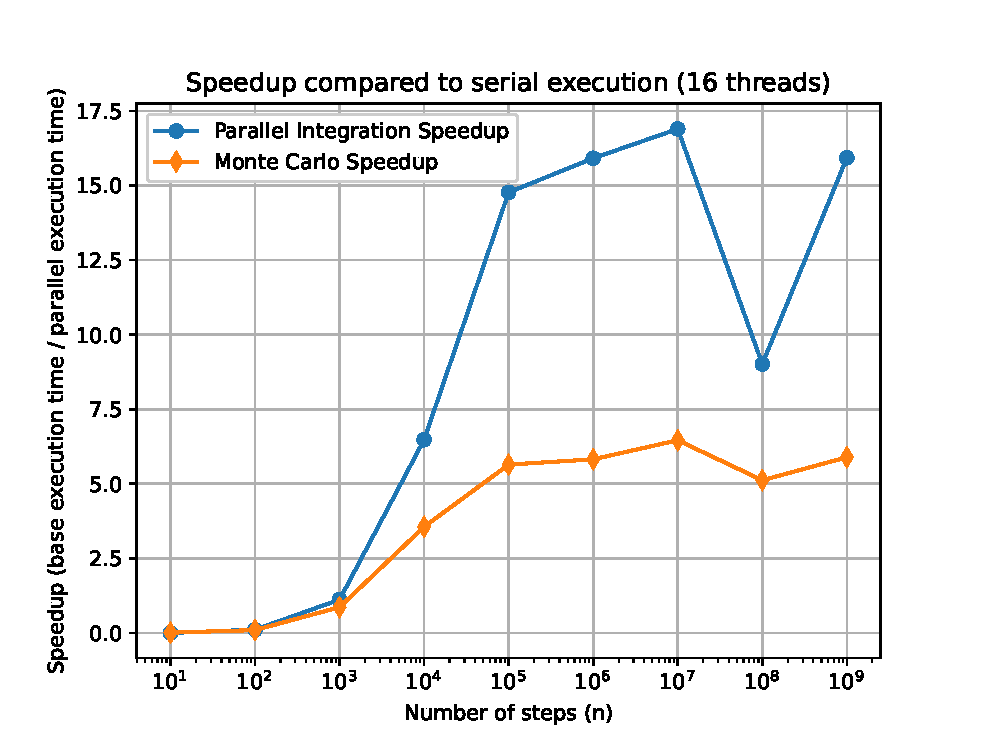
\includegraphics[height=6cm]{speedup.eps}
\caption{Speedup of both parallel methods compared to the serial integration function.}
\label{fig5}
\end{center}
\end{figure}

The graph is only computed for 16 threads, since (per figures three and four), that thread count produced optimal results for both parallel functions. Parallel integration experiences significantly more speedup than the Monte Carlo method. However, there is a bizarre dip in speedup at $n = 10^8$, which should be explored further. 
\\\\\\
\section{Results}
Overall, this report has shown that parallelized computation of pi using the integration method is much more efficient than either the parallel integration method or the parallel Monte Carlo method, and is more accurate than the Monte Carlo method. Both parallel functions scale well with increased thread count.

It should be noted that the computation for this report was completed on ix-dev, which (to my knowledge) is not optimized for parallel computing. This report should be compared with the results found by my peers to better understand what these methods look like when running on Talapas. Additionally, there are likely paralleization optimizations that I have not tried or considered, so this should be considered simply an initial stab at analysis. I would also be interested in running more tests, increasing both the number of tests done at each thread count and the maximum n evaluated. 


\end{document}


